%\documentclass[a4paper,12pt]{book}
%\usepackage{fixltx2e}
%\usepackage{graphicx}    
%\begin{document}
\chapter{Background Study and Related Works}
\lhead{Chapter 2. \emph{Background Study and Related Works}}
In this chapter, we have described some related works and provide some background stuffs those are appropriate to the remainder of this paper. We have discussed different terminology and related analysis for better understanding. We have focused the recent research works on uncertain and stream database. We have provided the analysis of existing algorithms, approaches their philosophy, working procedure, complexity analysis, aim and limitations that will help very much for better understanding and improvement of existing approaches.

\section{Data Mining}
In the previous chapter, Chapter 1 Introduction, we have described regarding data mining, frequent pattern mining over certain data, uncertain data, stream data and uncertain stream data. Basically, frequent pattern from any sort of data follows two approaches. First one is candidate generation and test-based approach named Apriori ~\cite{apriori}. Second one is pattern growth approach named as FP-growth ~\cite{fp_growth}. Apriori ~\cite{apriori} is a prior knowledge based algorithm, that is, if any pattern is not frequent then one of its super-patterns must not be frequent. It works in a level-wise approach. From the given database in each level, it generates frequent sub-patterns and merges them to propagate the candidates for next level. In this approach, multiple times scan of the database is mandatory and, a lot of test cases needed to be tested and for each check it is mandatory to search the database again and again. On the other hand, FP-growth ~\cite{fp_growth} has been adopted the divide and conquer approach. This has solved multiple scans and also reduced the huge candidate test. In this approach, firstly the huge database is compressed and put into a data structure named FP-tree holding the item-set association information and divide such a compressed database into a set of condition databases, each associated with one frequent item, and mine the constructed conditional database recursively. Here, there is no need to generate the candidate for next level or no need to generate candidate. Apriori suffers from huge candidate generation whereas FP-growth has resolved this problem. However, Apriori ~\cite{apriori} suffers much more when support factor. Thus, all the approaches derived or influenced by Apriori ~\cite{apriori} (e.g. U-priori ~\cite{u_priori}) also suffers from this problem.

\section{Uncertain Stream Data}
Data uncertainty is an inherent property in various applications due to reasons such as hardware fault, the uncertainty of incidents, outdated sources or imprecise/incorrect measurement. In the age of big data, uncertainty is one of the defining characteristics of data. Data is constantly growing in volume, variety, velocity and uncertainty. In a large range of applications domains uncertain data is found in abundance. Today on the World Wide Web, data from sensor networks like GPS, weather detection machines, within enterprises both in their structured and unstructured sources, biological data, meteorological trends, of the medical behavior of living organisms’ data, human behavior, are the example of uncertain data. Customer name of a super shop is a real life example of uncertain data. For example, there exist several customers named Mrs./Mr X registered in a super shop but if we want a particular Mrs./Mr. X then we will not certainly be able to find her/him by name.\\ \\
In the modern age, there are much more instruments we are being used to like smart-phones, smart-gears (e.g. smart watch, smart glass). All the devices have many more sensors those are collecting data each and every micro second. But all the data from the sources are imprecise or incorrect. For example, a temperature sensor gives some information like current temperature is 40 degree, with 5\%-10\% error. This makes this data imprecise and uncertain. Moreover, features like weather forecast are inherently uncertain. For example, today's weather forecast may be rainy but it has only 65\% confidence. There are many cases when information acquired from human experiences is not reliable and precise. Different people can describe the same incident in different view and perspective. As an example, in a bird viewing event Mr. C saw a crow flying by. But, Mr. D thinks it was a raven. So, uncertainty values can be attached with these observations like the bird has 75\% probability to be crowd and 20\% probability to be a raven.
%\documentclass{article} 
%\usepackage{graphicx}  
%\usepackage{multirow}
%\usepackage[table]{xcolor}
%\usepackage{fixltx2e}
%\usepackage{array}
%
%\begin{document}
\begin{table}[ht]
\centering

\begin{tabular}{|c|c|c|c|c|c|}
\hline
	Transaction No & \multicolumn{4}{c|}{Items in Transaction} \\ \hline \hline
	T\textsubscript{1} & a(0.9) & c(0.6) & d(0.5) & e(0.2)			\\\hline
	T\textsubscript{2} & a(0.9) & b(0.4) & e(0.1) & --    			\\\hline
	T\textsubscript{3} & a(0.2) & c(0.9) & d(0.7) & --    			\\\hline
	T\textsubscript{4} & b(0.3) & c(0.9) & -- & --			\\\hline
	T\textsubscript{5} & a(0.1) & b(0.3) & c(0.9) & --    			\\\hline
	T\textsubscript{6} & a(0.9) & e(0.3) & -- & --        			\\\hline
   	T\textsubscript{7} & a(0.1) & d(0.6) & e(0.2) & --		\\\hline
	T\textsubscript{8} & a(0.1) & c(0.2) & f(0.6) & --    			\\\hline
	T\textsubscript{9} & c(0.2) & d(0.9) & f(0.6) & --    			\\\hline
	
	T\textsubscript{10} &  --  &  --  &  --  & --    				\\\hline
	T\textsubscript{11} &  --  &  --  &  --  & --    				\\\hline
	T\textsubscript{12} &  --  &  --  &  --  & --    				\\\hline
	
		
\end{tabular}
\label{tab:ex_u}
\caption{Example of Uncertain Stream Transaction}
\label{table:uncertain_stream_transaction}
\end{table}
%\end{document}
\subsection{Categorization of Uncertain Data}
By type of uncertainty assignment, uncertain data can be categorized into three types. They are:
\paragraph{Attribute Uncertainty}
In attribute uncertainty, each uncertain attribute in a tuple has its own independent probability distribution. For example, if readings are taken of temperature and wind speed, each would be described by its own probability distribution for correctness and precision, as knowing the reading for one measurement would not provide any information about the other.
\paragraph{Correlated Uncertainty}
In correlated uncertainty, multiple attributes may be described by a joint probability distribution. For example, if rain occurs, then a musical festival event will be stopped. Then the occurrence of the event depends on the probability of rain. And thus this makes a co-relation with rain and musical festival
\paragraph{Tuple Uncertainty}
In tuple uncertainty, all the attributes of a tuple are subject to a joint probability distribution. This covers the case of correlated uncertainty but also includes the case where there is a probability of a tuple not belonging in the relevant relation, which is indicated by all the probabilities not summing to one. For example, assume we have a tuple $T_i = (a, 0.4) - (b, 0.5)$ and the probability this tuple exists in the database is 10\%. Then this is called tuple uncertain.
        \begin{figure}
        \centering
            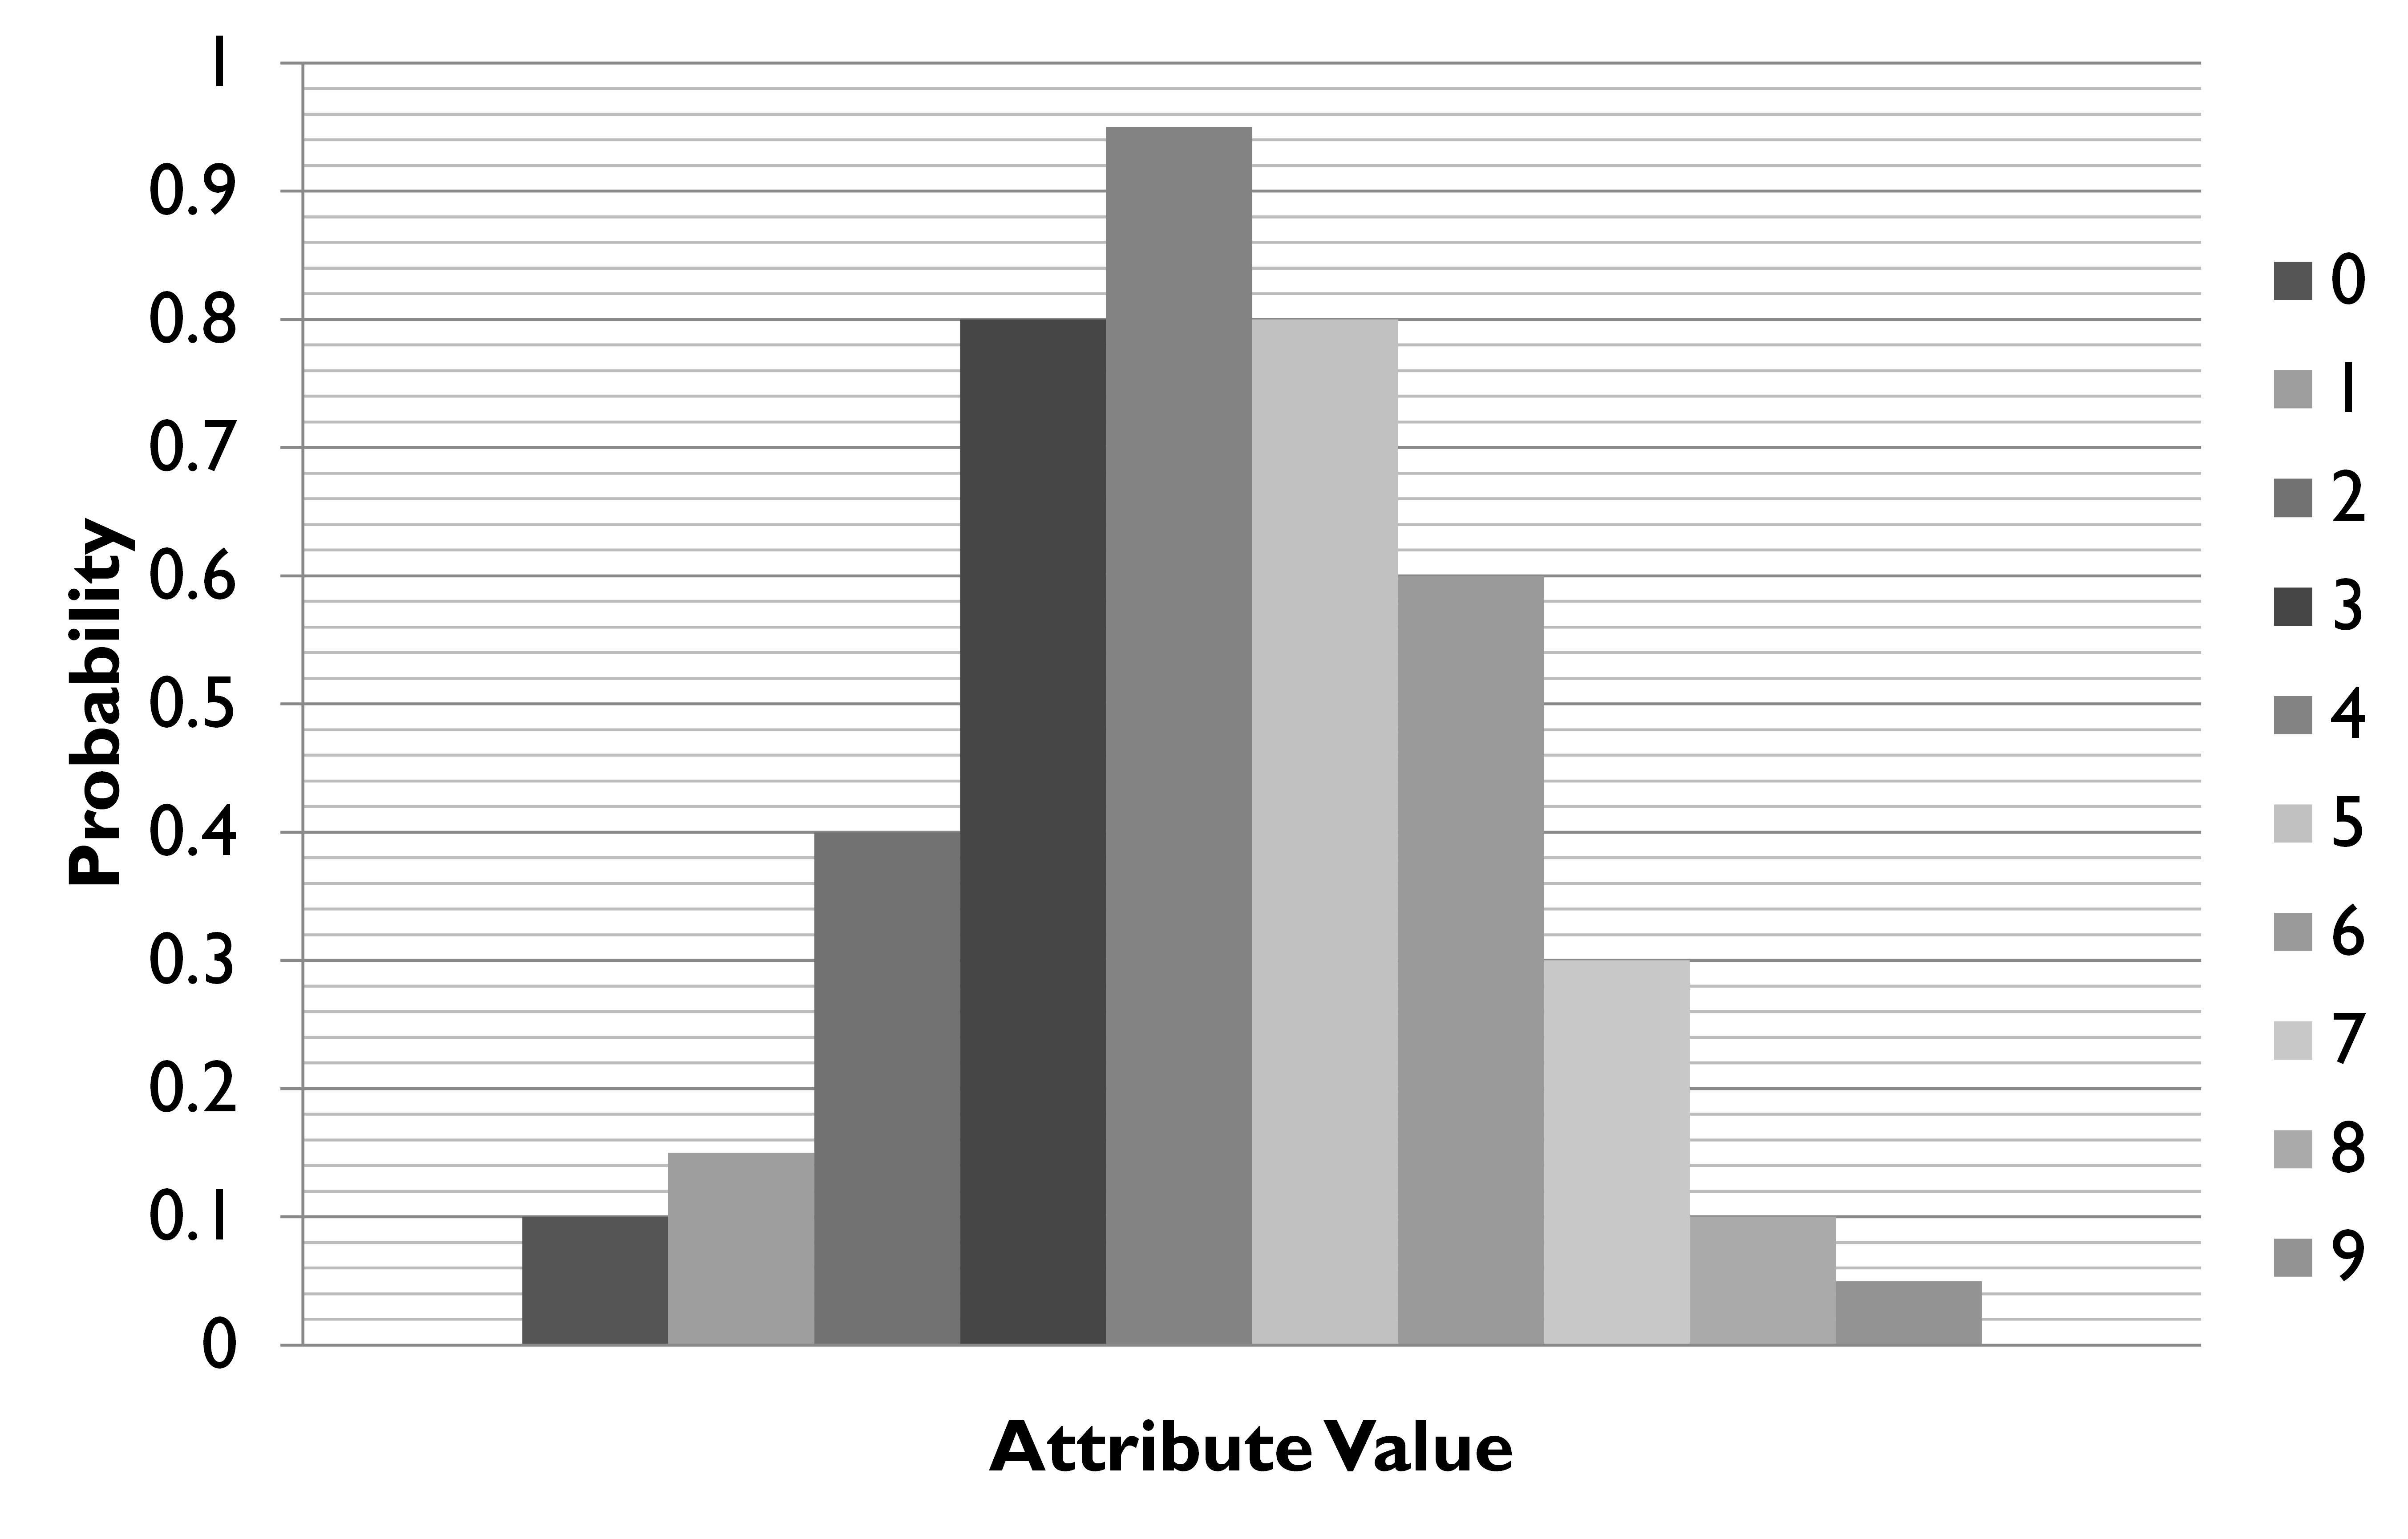
\includegraphics[width=1\textwidth]{../images/d_probability}
        \caption{Discrete Probability Distribution}
        \label{figure:d_probability}
        \end{figure}
        \begin{figure}
        \centering
            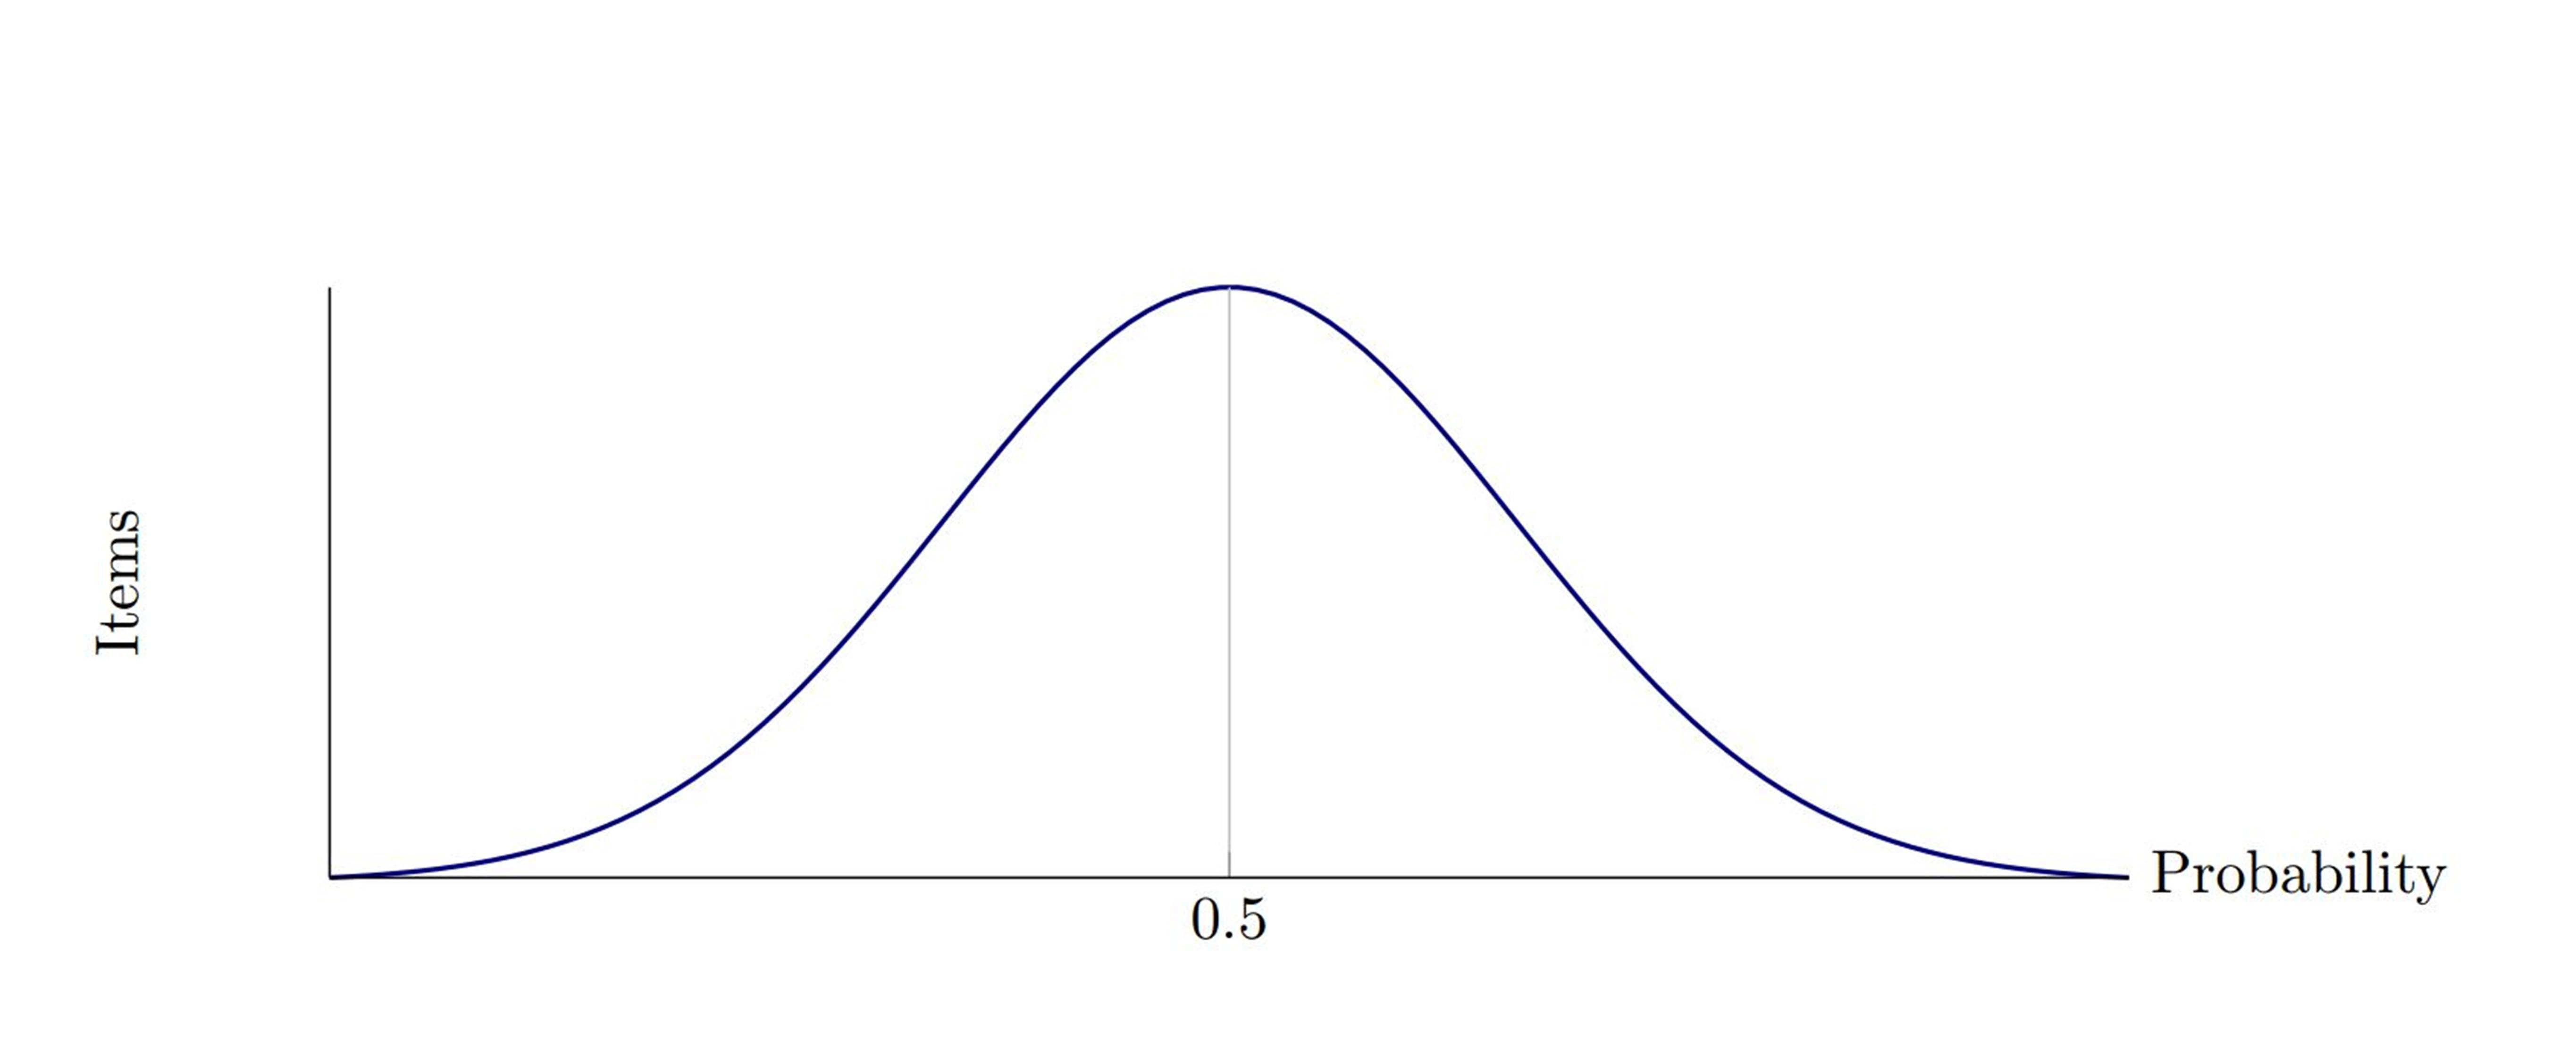
\includegraphics[width=1\textwidth]{../images/c_probability}
        \caption{Continuous Probability Distribution}
        \label{figure:c_probability}
        \end{figure}
\subsection{Uncertainty Types}
Uncertainty can be of two types: discrete and continuous. In this uncertainty the probability of an uncertainty is discrete value (figure \ref{figure:d_probability}). Continuous uncertainty means the probability of an item/event being certain lies between a certain value (e.g. 0 and 1 figure \ref{figure:c_probability}). In many real-life applications, uncertain objects are already given by discrete observations, in particular if the objects are derived from sensor signals. This type of representation is motivated by the fact, in many cases, only discrete but ambiguous object information as usually returned by common sensor devices is available, for example discrete snapshots of continuously moving objects.

\subsection{Expected Support for Uncertain Data}
For uncertain data expected support calculation is not straightforward. The support calculation follows the following equation.
    \begin{equation}
expSup \qquad = \qquad \sum_{i = 0}^{UDB} [\prod_{x \in I } p(x , t_i)]
    \end{equation}
\emph {where,}    \textbf{\emph {I}} is item-set,    \textbf{\emph { p(x, ti)}} is existential probability value for any item \textbf{\emph {x}} in transaction \textbf{\emph {t\textsubscript{i}}} \textbf{\emph {UDB}} is an uncertain database.\\
For example let table \ref{table:uncertain_stream_transaction} be consider a uncertain database. Here expected support of item-set \emph{ab} will be $0+0.9*0.4+0+0+0.3*0.1+0+0+0+0=0.39$.

\subsection{Stream Data}
Stream data is data unbounded and continuous data incoming from any data sources that is producing all time the lots of data. These data is that much continuous and extreme in volume that storing this much data in any storage cannot be thought. This much data processing and storing make a huge cost that can think. This stream of data is valueless unless this is processed, categorized and extract important knowledge. But this garbage can be diamond if this data is categorized and extract important information. Here data mining plays an important role.\\ \\
For example, day by day with the enormous increase of internet availability and use the data producing each day by each user in every micro second is extremely huge. This big data computation is much more difficult. Particularly we can look at an example: as the social media is being popular day by day people are using these media like Facebook ~\cite{facebook}, Twitter \cite{twitter} etc. They are being used to these medias. Passing much more times and this gives a great opportunity to get very much valuable information regarding their likes, their daily routine, their current status, their friends, and families. This gives much more opportunity to profile people, categorized them. This gives the service selling organizations a great scope to digital online marketing, advertising their products and offer many promotional offers to people. Again, as this is used to communicate with each other than any terrorist activity can be predict earlier from these resources found from the web. But the main difficulty is to extract information to categorized and profile these extreme data incomings from source.

\section{Existing Approaches}
Many algorithms have been developed to mine frequent item-sets from uncertain databases. Among them, some are Apriori ~\cite{apriori} like approach and others are FP-growth ~\cite{fp_growth} like approach. U-Apriori ~\cite{u_priori} was proposed to mine uncertain frequent pattern that is Apriori-like candidate generation and test-based approach. UF-growth ~\cite{uf_growth}, UFP-growth ~\cite{ufp_growth} was proposed to mine frequent patterns from uncertain data but this suffers much more for compactness of tree. CUF-growth ~\cite{cuf_growth}, CUF-growth\textsuperscript{*} ~\cite{cuf_growth}, PUF-growth ~\cite{cuf_growth} was proposed later for mining uncertain data but they produce false positives as they works with probabilistic uncertainty modeling. All of them are unable to mine stream of uncertain data. UF-stream ~\cite{suf_growth} and SUF-growth ~\cite{suf_growth} proposed to mine uncertain frequent pattern from stream. UF-stream ~\cite{suf_growth} suffers from both false positives and false negatives. The SUF-growth ~\cite{suf_growth} is an exact mining algorithm that has resolved the false positive and false negative generation but the constructed tree structure is like UF-growth ~\cite{uf_growth} that suffers much because the data structure (tree) SUF-growth ~\cite{suf_growth} use to keep information is not compact. Before elaborate discussion of SUF-growth ~\cite{suf_growth} we will provide a brief discussion on the background of uncertain stream mining approaches.
    
    
    \subsection{U-Priori}
    U-Apriori ~\cite{u_priori} is a modification of Apriori ~\cite{apriori} algorithm which is proposed to handle uncertain data. We already know in Apriori ~\cite{apriori} algorithm support count play an important role. A number of databases scan and candidate for next level depends on support count. The modification of Apriori in U-Apriori is supporting count. It has designed for handling support using minimum support calculation of uncertain data. Instead of incrementing the support counts of candidate patterns by their actual support, U-Apriori increments the support counts of candidate patterns by their given support count using the uncertain support count equation. Though U-Apriori comes over Apriori to solve support count problem of uncertain data but U-Apriori suffers from the some problems. As U-Apriori is a modification of the Apriori algorithm, performance of U-Apriori algorithm for large scale of data because it follows level wise sub-patterns generation and merge to generate the candidate for next level. That's why the number of databases scans increase with the dimension of the item-set. If the existential probabilities of most items within a pattern $I$ are small, increments for each transaction can be insignificantly small. Consequently, many candidates would not be recognized as infrequent until most transaction was processed.  
    
    \subsection{UF-growth}
    Observing outperforms of FP-growth ~\cite{fp_growth} over Apriori ~\cite{apriori}, UF-growth ~\cite{uf_growth} was proposed for mining uncertain data. We know the key to the success of FP-growth over Apriori is FP-tree, which is a compact tree structure capturing frequent items within transactions in the databases of precise data. Like FP-growth, UF-growth also used the tree construction approach. This constructs UF-tree By extracting appropriate tree paths to construct subsequent FP-trees, frequent item-set can be mined. Each tree path represents a transaction. Each node in a tree path captures (i) an item x and (ii) its actual support (i.e., occurrence count of x in that tree path). Tree paths (from the root) are merged if they share the same items (i.e., the captured two items share a node if they have both same item id and same existential probability). Due to this path sharing, the UF-tree is usually compact. However, as dealing with uncertain data, the situation is different from certain data. The expected support of any item-set X is the sum of products of the existential probability of items within X. Hence, UF-growth uses a UF-tree to capture frequent items within transactions of uncertain data. Each node in a UF-tree captures (i) an item x, (ii) its existential probability value, and (iii) the occurrence count of x in that tree path. By doing so, UF-growth finds all and only those frequent item-sets by computing the expected support of an item-set X (as the sum of products of the captured existential probability values). Tree paths are merged if they share the same items and existential probability values. Consequently, UF-trees may not be as compact as FP-trees. In real life scenario, this tree is never compact. And mining suffers much more as the candidate for sub-pattern tree grows as the transaction grows.
    
    \subsection{UFP-growth}
    To reduce the tree size in UF-tree of UF-growth ~\cite{uf_growth}, UFP-growth ~\cite{ufp_growth} was proposed. In this approach, items are grouped and share the same node (i.e., nodes with the same x but similar existential probability values) into a cluster. Each cluster of the item x captures (i) the maximum existential probability value of all nodes within the cluster and (ii) the number of existential probability values in each cluster. Depending on the clustering parameter, the resulting tree namely, UFP-tree may be as large as the UF-tree (i.e., no reduction in tree size). On the other hand, if the UFP-tree  is smaller than the UF-tree, then UFP-growth may return approximate results (e.g. with false positives or infrequent item-sets). Though it solves some tree compactness problem but the tree is still not that much compact. Moreover, this does not fit for uncertain stream data. 
    
    \subsection{PUF-growth}
    To reduce the size of the UF-tree ~\cite{uf_growth} and UFP-tree ~\cite{ufp_growth}, the prefix-capped uncertain frequent pattern tree, PUF-tree structure, and mining algorithm PUF-growth ~\cite{puf_growth} was proposed, in which important information about uncertain data is captured so that frequent patterns can be mined from the tree. The PUF-tree  is constructed by considering an upper bound of existential probability value for each item  which is named as I\textsuperscript{cap}. When generating a k-item-set (where $k>1$). This upper bound of an item x\textsubscript{r} in a transaction t\textsubscript{j} is called the (prefixed) item cap, I\textsuperscript{cap} of x\textsubscript{r} in t\textsubscript{j}. Thus, PUF-tree is very much compact. This approach generates some false positive. But the false positive reduction technique makes this a stronger approach. But this is not fit for uncertain stream data. 
    
    \subsection{UF-streaming}
    UF-streaming ~\cite{suf_growth} was proposed to mine frequent item from uncertain stream data. This is a sliding window approach, that capture most recent data, as most recent data is most important. It has divided the transaction stream data in several batch each batch is inserted into the tree structure that is UF-tree ~\cite{uf_growth} and mine each tree using UF-growth ~\cite{uf_growth} and put all the frequent patterns found in a UF-stream structure. For avoiding false negative they have used a value \emph{preMinSup} less than minimum support (0 < \emph{preMinSup}< minimum support). Then until the window is completed the frequent item-set is put into UF-stream tree structure. This has addressed the problems of stream uncertain data mining, but it suffers from some problems given below.
    \begin{itemize}
        \item Un-necessary mining each batch. Let window size is 3 and batch size is 2. If one wants the mining result at window 50 then in this approach it is needed to mine each of 1 to 50 batchs for getting the result.
        \item The used tree structure is UF-tree that suffers from compactness problem.
        \item Extra data structure for keeping frequent item-set UF-stream tree structure.
        \item False positive generation in the mining process.
        \item False negative generation in the mining process.
        \item This has high running time and memory consumption.
    \end{itemize}
    
    \subsection{SUF-growth}
    SUF-growth ~\cite{suf_growth} addressed the limitations exist in UF-streaming ~\cite{suf_growth}. SUF-growth algorithm outperforms over UF-streaming algorithm. It improves over UF-streaming by avoiding the aforementioned potential problems for mining frequent item-set from streams of uncertain data. SUF-growth is an exact algorithm. Its means SUF-growth returns only truly frequent item-set. Where UF-streaming returns both true and false frequent item-set. It uses the only \emph{minsup}. No need to use \emph{preMinsup}. There also have any problem of finding an appropriate value of \emph{preMinsup}. This algorithm does not need UF-stream structure to store the mined item-sets. Need transaction databases in memory resident for assumed performance. Instead of this its use delayed mode for mining. As a result, unnecessary computation could be reduced and unnecessary mining is avoided.
        \begin{figure}[]
        \centering
            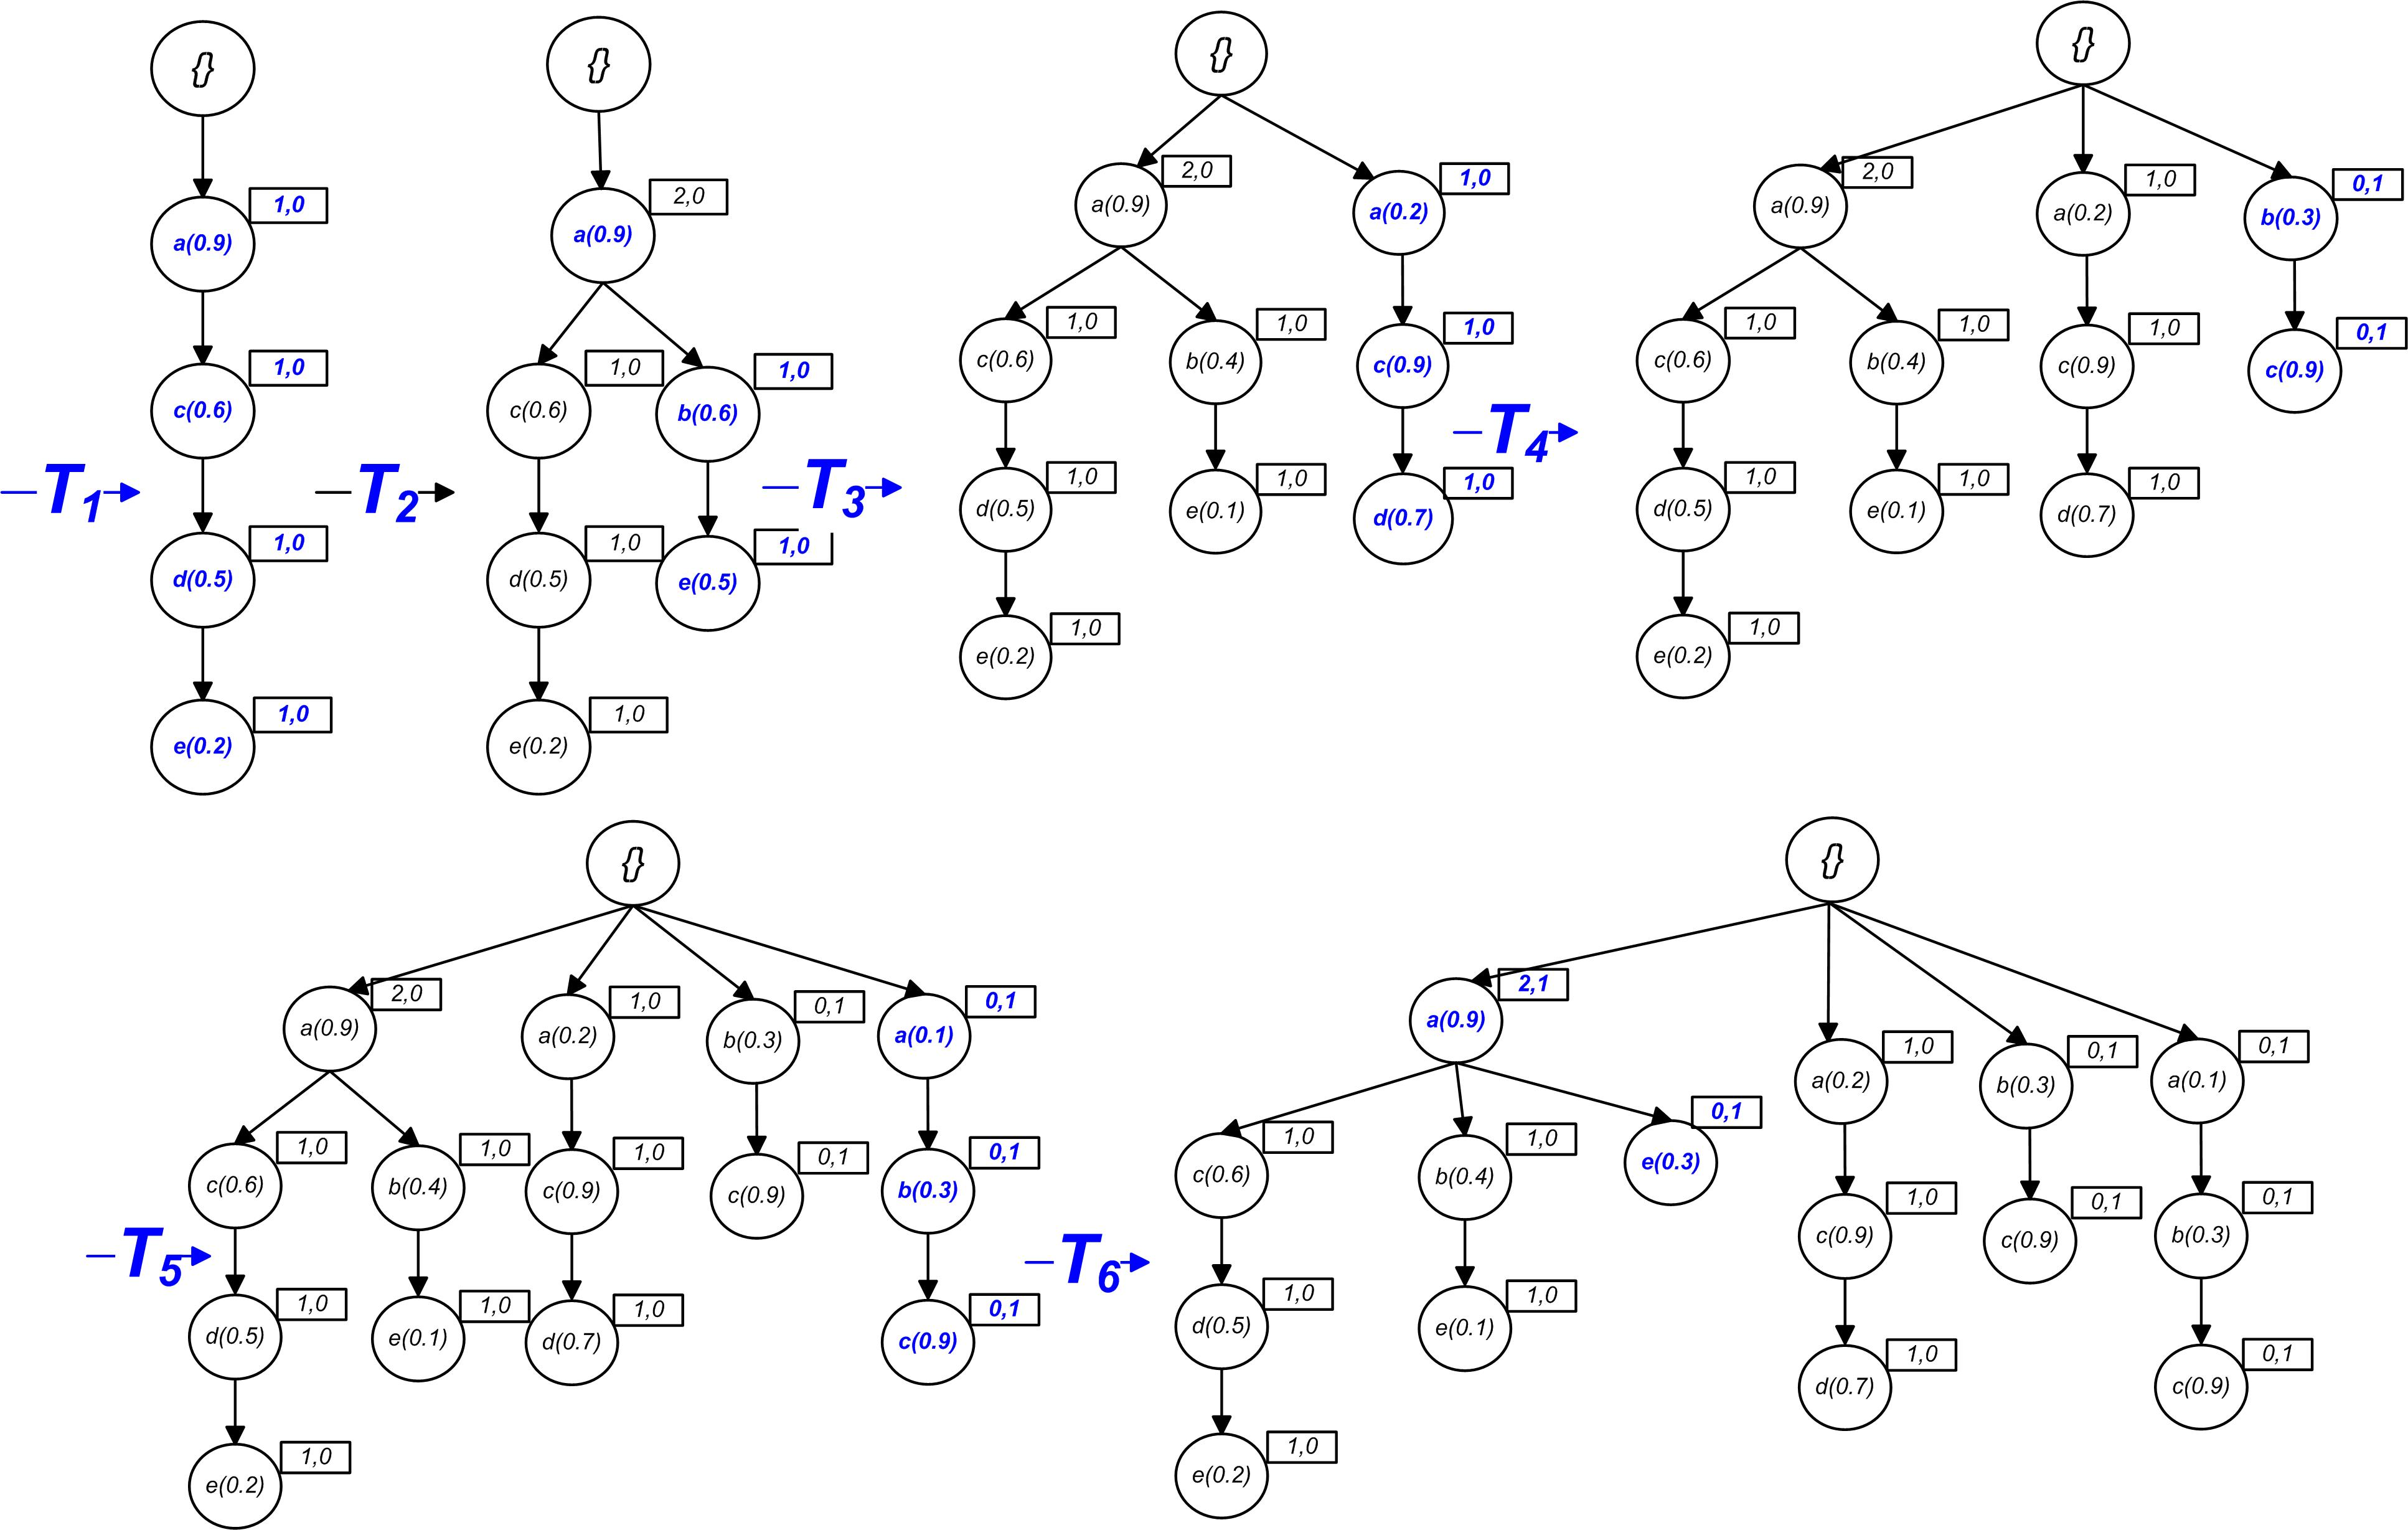
\includegraphics[width=1\textwidth]{../images/suf_simulation}
        \caption{SUF-growth ~\cite{suf_growth} tree construction}
        \label{figure:suf_simulation}
        \end{figure}
    Considering the advantages of SUF-growth over others algorithm, there is the question. The is how SUF-growth ~\cite{suf_growth} algorithm find frequent item-sets from streams of uncertain data using a new tree structure called SUF-tree. Now we describe this. We first construct an SUF-tree, and then extract relevant paths from this SUF-tree (which is a global tree) to recursively from smaller UF-trees for projected databases. Due to the dynamic nature and Property 2 of data streams, expected the support of items is continuously affected by the arrival of new batches (and the removal of the contents of older batches). Arranging items in the frequency-dependent order in the SUF-tree may lead to swapping which, in turn, can cause merging and splitting—off tree nodes when the global frequencies of items change. Hence, in the SUF-tree, items are arranged according to some canonical order (e.g. lexicographic order), which can be specified by the user prior to the construction of the SUF-tree or the mining process. Consequently, the SUF-tree can be constructed using only one scan of the streams of uncertain data, and the resulting SUF-tree captures the contents of the streams. Moreover, the SUF-tree preserves the usual tree properties. The occurrence count of a node is at least as high as the sum of occurrence counts of its children.The ordering of items is unaffected by the continuous changes in the expected support values of items.\\ \\
    For example for table \ref{table:uncertain_stream_transaction} transaction database let construct the SUF-tree. Figure \ref{figure:suf_simulation} shows the construction of the SUF-tree. Here as the stuff tree is based on UF-tree construction approach the node sharing is very rare. From figure \ref{figure:suf_simulation} it’s clearly visible that the node sharing is not that much impressive as the node should be shared if the two same item has same existential probability and in real life scenario this sharing is very rare. For this reason \emph{a(0.9)} in \emph{T\textsubscript{1}} and \emph{a(0.2)} in \emph{T\textsubscript{3}} did not share single node and the tree compactness could not be accomplished.
    Although the SUF-growth has resolved some limitations of UF-streaming ~\cite{suf_growth}, some limitations still exist. The findings are listed below:
    \begin{itemize}
        \item The tree structure it uses is UF-tree ~\cite{uf_growth} structure which suffers from compactness. So SUF-growth tree also inherits this limitation.
        \item The tree construction cost will be much more (both running time and memory) as the transaction grows.
        \item The mining algorithm it uses is FP-growth like the approach that generates a huge candidate sub-pattern tree that costs much in the mining time. It increased mining cost (both running time and memory).
     \end{itemize}
    
\section{Summary}
The approaches for finding frequent patterns on uncertain data is challenging because of data uncertainty property. Although many of the approaches has been adopted to address and solve this constraint but still there are limitations. Moreover, there are still limitations in mining uncertain stream. The compressed data structure design is a tough challenge for uncertain stream data. Later chapters we will provide a novel, completely new and efficient data structure that will make the tree compactness more and gain both running time and memory efficiency.
%\end{document}
